% !TEX root = BA-Bauer.tex

\subsection{Spannungsversorgung}
Eine stabile und zuverlässige Spannungsversorgung ist für jede Schaltung besonders wichtig, denn die beste Schaltung funktioniert nicht ohne sie. Um eine großtmögliche Kompatibilität für den Benutzer zu gewährleisten, wird das Gerät über eine USB-Schnittstelle mit der nötigen Spannung versorgt. Dadurch kann das Gerät von mobilen Akkus oder USB-Netzteilen betrieben werden. Die nachstehende Tabelle zeigt den benötigten Versorgungsspannungs- und den Strombedarf der einzelnen Komponenten. 
\begin{table}[h]
	\begin{center}
		\begin{tabular}{l | c | r }
			\textbf{Bauteil} & \textbf{Versorgungsspannung} & \textbf{Strombedarf}\\
			\hline
			MCU & 1,7\,V - 3,6\,V & max. 240\,mA\\
			RS485 Treiberchip VDDA & 1,71\,V - 5,5\,V & max. 6,6\,mA\\
			RS485 Treiberchip VDDB & 4,5\,V - 5,5\,V (isoliert)& max. 12,5\,mA\\
			DC/DC Konverter & 4,5\,V - 5,5\,V & 28\,mA\\
			LCD-Modul & 3\,V - 10\,V & 100\,mA\\
			LED & 5\,V & ca. 20\,mA\\
			SD-Kartensteckplatz & 3,3\,V & -\\
			Encoder & 5\,V & -\\
			Taster & - & -\\
			\hline
			\textbf{Gesamt} & - & max. ca. 481\,mA
		\end{tabular}
	\caption{Spannungs- und Strombedarf}
	\label{tab:VDD+IDD}
	\end{center}
\end{table}
Die USB-Schnittstelle liefert laut der USB2.0-Spezifikation zwischen 4,75\,V und 5,5\,V \cite[s. 283]{USB-PD} und standardmäßig einen Strom von 100\,mA. Um mehr Strom von einem USB-Host\footnote{In der Hierarchie übergeordnetes USB-Gerät} anzufordern ist eine Kommunikation über die USB-Datenleitungen mithilfe eines Mikrocontrollers oder einem speziell für diesen Zweck vorgesehenen Chip notwendig. Allerdings kann das Gerät durch das Verbinden der beiden USB-Datenleitunen \textit{D+} und \textit{D-} mit einem Widerstand kleiner 200\,$\Omega$ als \textit{dedicated charging port} (DCP) registriert werden \cite[s. 41]{USB-Battery}. Durch die Einstufung als DCP kann der USB-Host ohne jegliche Kommunikation bis zu 1,5\,A freigegeben \cite[s. 45]{USB-Battery}. Als Stromversorgung können dann einfache USB-Netzteile, mobile -Batterien, -Anschlüsse an Laptops und PCs, sowie HUBs mit einer externen Stromversorgung genutzt werden.Voraussetzung für die Lieferung des Stroms ist eine ausreichende Stromversorgung des USB-Host selbst. 
\begin{figure}[h]
	\begin{center}
		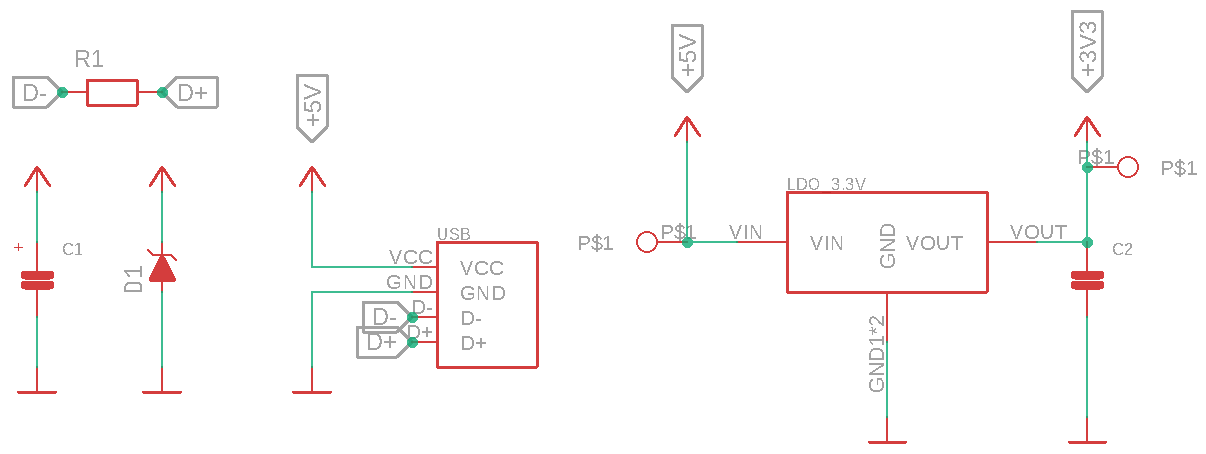
\includegraphics[width=.8\linewidth]{Schaltung-power}	
		\caption{Schaltung Spannungsversorgung}
		\label{fig:Schaltung-power}
	\end{center}
\end{figure}
Abbildung \ref{fig:Schaltung-power} zeigt die Schaltung der Spannungsvergung der Schaltung. Der Widerstand $R1$ sorgt dafür, dass das Gerät als DCP erkannt wird. Der Elektrolyt-Kondensator $C1$ fundiert als kleiner Puffer, falls die Schaltung für einen kurzen Moment mehr Strom benötigt als die USB-Schnittstelle liefern kann. Der damit einhergehende Spannungsabfall wird zudem kurzzeitig ausgeglichen. Um eventuell zurückfließenden Strom in den USB-Host zu verhindern wird die Diode $D1$ parallel zum 5\,V Potential (VCC) und Ground (GND) geschaltet. Auf der rechten Seite der Abbildung \ref{fig:Schaltung-power} befindet sich ein LDO-Spannungsregler. Er regelt die eingehenden 5\,V vom USB-Host auf 3,3\,V herunter und stabilisiert diese gleichzeitig. Laut Tabelle \ref{tab:VDD+IDD} wird ein Strom von maximal ca. 240\,mA aus dem Spannungsregler erwartet. Laut Datenblatt fällt an ihm bei 25\,$^{\circ}$C und einem Strom von 250\,mA eine Spannung von ca. 100\,mV ab. Der MCU und der SD-Kartensteckplatz können somit mit ausreichend Spannung versorgt werden. Alle anderen Komponenten werden direkt mit den 5\,V der USB-Schnittstelle versorgt um den LDO-Spannungsregler so wenig wie möglich zu belasten.